\section{Notation and Basic Concepts}\label{cha:TensorNetworks}

We here provide the fundamental definitions of tensors, which are essentiell for the content in \parref{par:one} and \parref{par:two}.
In \parref{par:three} we will further investigate the properties of tensors focusing on their contractions.

\subsection{Categorical Variables and Representations}

We will in this work investigate systems, which are described by a set of properties, each called a categorical variable. 
This is called an ontological commitment, since it defines what properties a system has.

\begin{definition}
	An atomic representation of a system is described by a categorical variables $\catvariable$ taking values $\catindex$ in a finite set 
		\[  [\catdim]\coloneqq \{0,\ldots, \catdim-1\} \]
	of cardinality $\catdim$.
\end{definition}

% Notation: Large and small literals
We will in this work always notate categorical variables by large literals and indices by small literals, possible with other letters such as $\catvariable,\selvariable,\indvariable,\datvariable$ and corresponding values $\catindex,\selindex,\indindex,\datindex$.

\begin{definition}
	A factored representation of a system is a set of categorical variables $\catvariableof{\atomenumerator}$, where $\atomenumeratorin$, taking values in $[\catdimof{\atomenumerator}]$.
\end{definition}

\subsection{Tensors}

% Gentle introduction sentences
Tensors are multiway arrays and a generalization of vectors and matrices to higher orders.
We will first provide a formal definition as real maps from index sets enumerating the coordinates of vectors, matrices and larger order tensors.

\begin{definition}[Tensor]\label{def:tensor}
	Let there be numbers $\catdimof{\atomenumerator}\in\nn$ for $\atomenumeratorin$ and categorical variables $\catvariableof{\atomenumerator}$ taking their values in $[\catdimof{\atomenumerator}]$.
	We call maps
	\begin{align*}
		\hypercoreat{\catvariables} : \bigtimes_{\atomenumeratorin} [\catdimof{\atomenumerator}] \rightarrow \rr
	\end{align*}
	tensor of order $\atomorder$ and leg dimensions $\catdimof{0},\ldots,\catdimof{\atomorder-1}$.
	Evaluations of these maps at indices $\catindices$ are denoted by
	\begin{align*}
		\hypercoreat{\indexedcatvariables} = \hypercoreat{\catvariables}(\catindices) \, .
	\end{align*}	
%	with coordinates denoted by $\hypercore_{\catindices}$ is called a tensor of order $\atomorder$ and legs with the dimensions $\catdimof{0},\ldots,\catdimof{\atomorder-1}$.
	Tensors $\hypercoreat{\catvariables}$ are elements of the space
	\begin{align*}
		\bigotimes_{\atomenumeratorin} \rr^{\catdimof{\atomenumerator}} \,  
	\end{align*}
	which is, with the operations of coordinatewise summation and scalar multiplication, a linear space called a tensor space.
\end{definition} 

% Non-canonical 
We here introduced tensors in a non-canonical way based on categorical variables assigned to its axis.
While coming as syntactic sugar at this point, this will allow us to define contractions without further specification of axes, based on comparisons of shared categorical variables.
Especially, this eases the implementation of tensor network contractions without the need to further specify a graph (see Appendix~\ref{cha:implementation}).

% Further abbreviations
We abbreviate lists $\catvariables$ of categorical variables by $\shortcatvariables$, that is denote $\hypercoreat{\catvariables}$ by $\hypercoreat{\shortcatvariables}$.
Occasionally, when the categorical variables of a tensor are clear from the context, we will omit the notation of the variables. %further abbreviate $\hypercoreat{\catvariables}$ by $\hypercore$.

\begin{example}[Trivial Tensor]\label{exa:trivialTensor}
	The trivial tensor is defined as the map 
		\[ \onesat{\shortcatvariables} : \facstates \rightarrow \{1\} \subset \rr \]
	with all coordinates being $1$, that is for all $\catindices\in\facstates$
		\[ \onesat{\indexedshortcatvariables} = 1 \, . \]
\end{example}


\subsection{One-hot encodings}

We are now ready to provide the link between tensors and states of systems with factored representations.
To this end, we define the one-hot encoding of a state, which is a bijection between the states and the basis elements of a tensor space.

\begin{definition}[One-hot encodings to Atomic Representations]
	Given an atomic system described by the categorical variable $\catvariable$, we define for each $\catindex\in[\catdim]$ the basis vector $\onehotmapofat{\catindex}{\catvariable}$ by
	\begin{align}
		\onehotmapofat{\catindex}{\catvariable=\tilde{\catindex}} = \begin{cases}
			1 & \text{if} \quad \catindex=\tilde{\catindex} \\
			0 & \text{else} \, .
		\end{cases} 
	\end{align}
	The one-hot encoding of states $\catindex\in[\catdim]$ of the atomic system described by the categorical variable $\catvariable$ is the map
		\[ \onehotmap: [\catdim] \rightarrow \rr^\catdim \]
	which maps $\catindex \in [\catdim]$ to the basis vectors $\onehotmapofat{\catindex}{\catvariable}$.
\end{definition}

% Coordinatewise representation
The basis vectors $\onehotmapofat{\catindex}{\catvariable}$ are tensors of order $1$ and leg dimension $\catdim$ of the structure
\begin{align}
	\onehotmapofat{\catindex}{\catvariable} = \begin{bmatrix}
	0 & \cdots & 0 & 1 &  0 & \cdots & 0
	\end{bmatrix}^T \, ,
\end{align}
where the $1$ is at the $\catindex$th coordinate of the vector.

% Atomic -> Factored system
We have so far described one-hot representations of the states of a single categorical variable, which would suffice to encode the state of an atomic system.
In a factored system on the other side, we are dealing with multiple categorical variables.

\begin{definition}[One-hot encodings to Factored Representations]
	Let there be a factored system defined by a tuple $(\catvariables)$ of variables taking values in $\facstates$.
	The one-hot encoding of its states is the tensor product of the one-hot encoding to each categorical variables, that is the map
		\[ \onehotmap : \facstates \rightarrow  \facspace \]
	defined by mapping $\catindices=\shortcatindices$ to
	\begin{align*}
		 \onehotmapofat{\shortcatindices}{\shortcatvariables}
		=: \bigotimes_{\atomenumeratorin} \onehotmapofat{\catindexof{\atomenumerator}}{\catvariableof{\atomenumerator}} \, . 
	\end{align*}
	We will call one-hot representations \emph{tensor representations} and depict them as
	\begin{center}
		\begin{tikzpicture}[scale=0.35,thick] % , baseline = -3.5pt


\draw (-12,1) rectangle (-3,3);
\node[anchor=center] (text) at (-7.5,2) {\corelabelsize $\bigotimes_{\atomenumeratorin} \onehotmapof{\catindexof{\atomenumerator}}$};
\draw (-11,1)--(-11,-1) node[midway,right] {\colorlabelsize $\catvariableof{0}$};
\draw (-9.5,1)--(-9.5,-1) node[midway,right] {\colorlabelsize $\catvariableof{1}$};
\node[anchor=center] (text) at (-6.75,0) {$\cdots$};
\draw (-4,1)--(-4,-1) node[midway,right] {\colorlabelsize $\catvariableof{\atomorder\shortminus1}$};


\node[anchor=center] (text) at (-1,2) {\corelabelsize ${=}$};

\draw (1,1) rectangle (3,3);
\node[anchor=center] (text) at (2,2) {\corelabelsize $\onehotmapof{\catindexof{0}}$};
\draw (2,1)--(2,-1) node[midway,right] {\colorlabelsize $\catvariableof{0}$};

\node[anchor=center] (text) at (4.5,2) {$\otimes$};

\draw (6,1) rectangle (8,3);
\node[anchor=center] (text) at (7,2) {\corelabelsize $\onehotmapof{\catindexof{1}}$};
\draw (7,1)--(7,-1) node[midway,right] {\colorlabelsize $\catvariableof{1}$};

\node[anchor=center] (text) at (9.5,2) {$\otimes$};

\node[anchor=center] (text) at (11,2) {$\cdots$};

\node[anchor=center] (text) at (12.5,2) {$\otimes$};


\draw (14,1) rectangle (16,3);
\node[anchor=center] (text) at (15,2) {\corelabelsize $\onehotmapof{\catindexof{\atomorder\shortminus1}}$};
\draw (15,1)--(15,-1) node[midway,right] {\colorlabelsize $\catvariableof{\atomorder\shortminus1}$};





\end{tikzpicture}
	\end{center}
\end{definition}


\begin{remark}[Flattening of Tensors]
	The use the tensor product to represent states of factored systems can be motivated by the reduction to atomic systems by enumeration of the states.
	We have this property reflected in the state encoding of factored systems, since the tensor space $\bigotimes_{\atomenumeratorin}\rr^{\catdimof{\atomenumerator}}$ is isomorphic to the vector spaces $\rr^{\prod_{\atomenumeratorin}\catdimof{\atomenumerator}}$.
	This operation is called flattening (or unfolding) of tensors with many axes to tensors of less axes.
\end{remark}



\subsection{Contractions}

Contractions are the central manipulation operation on sets of tensors.
To introduce them, we will develop a graphical illustration of sets of tensors, which we also call tensor networks.
In \parref{par:three} we will further investigate the utility of contractions in representing specific calculations, which demand different encoding schemes.


\subsubsection{Graphical Illustrations}

% Hypergraph as capturing the categorical variable assignment to tensors
Sets of tensor with categorical variables assigned to each legs implicitly carry a notion of a hypergraph.
This perspective is especially useful, when some categorical variables are assigned to axis of multiple tensors, as it will often be the case in the applications considered in this work.
Each variable can then be labeled by a node and each tensor as a hyperedge containing the nodes to its axis variables.
Let us first formally introduce hypergraphs, which are generalizations of graphs allowing edges to be arbitrary nonempty subsets of the nodes, whereas canonical graphs demand a cardinality of two.

\begin{definition}\label{def:hypergraphs}
	A hypergraph is a pair $\graph=(\nodes,\edges)$ of a set of nodes $\nodes$ and a set of edges $\edges$, where each hyperedge $\edge\in\edges$ is a subset of the nodes $\nodes$.
	A directed hypergraph is a pair $\graph=(\nodes,\edges)$, such that each hyperedge $\edge\in\edges$ is the tuple of two disjoint sets $\incomingnodes,\outgoingnodes\subset\nodes$, that is
		\[ \edge = (\incomingnodes,\outgoingnodes)  \, . \]
\end{definition}

% Diagrammatic representation in factor graphs
We will use the standard visualization by factor graphs as a diagrammatic illustration of sets of tensors, where tensors are represented by block nodes and each axis assigned with by a categorical variable $\catvariableof{\atomenumerator}$ represented by a node, see Figure~\ref{fig:tensors}a). 
%We further denote on Each axis of the tensor is represented by a node representing the variable $\catvariableof{\atomenumerator}$ and the tensor $\hypercore$ is associated with the hyperedge $\edge$ connecting all variables.
 %representing the choice of an element in the set $[\catdimof{\atomenumerator}]$
% Hyperedge view
Different simplifications of these factor graph depictions have been evolved in different research fields.
In the tradition of graphical models, which started with the work \cite{pearl_probabilistic_1988}, the categorical variables are highlighted and the tensor blocks just depicted by hyperedges.
To depict dependencies with causal interpretations, the edges are further decorated by directions in the depiction of Bayesian networks, see for example \cite{pearl_causality_2009}.

In the tensor network community on the other hand, a simplification scheme highlighting the tensors as blocks and omitting the depiction of categorical variables has been evolved.
The variables, or sometimes their index or dimension, are then directly assigned to the lines depicting the axes of the tensor blocks.

Both depiction schemes are simplifications of factor graphs, by highlighting the categorical variables in the depiction in Figure~\ref{fig:tensors}b) and the tensors in the depiction in Figure~\ref{fig:tensors}c).
We in this work will prefer the simplification of the tensor network community, depicted in Figure~\ref{fig:tensors}b).

% Duality
In another interpretation (see \cite{robeva_duality_2019}), both simplification schemes are itself interpret as hypergraphs, which are dual to each other.

\begin{figure}[h!]
	\begin{center}
		\begin{tikzpicture}[scale=0.35,thick] % , baseline = -3.5pt


\begin{scope}[shift={(-17,0)}]

\node[anchor=center] (text) at (-3,0) {$a)$};

\draw (-1,1) rectangle (10,-1);
\node[anchor=center] (text) at (4.5,0) {\small $\hypercoreof{\edge}$};

\draw (0,-1)--(0,-3) node[midway,left] {\tiny $\catvariableof{0}$}; 
\draw (3,-1)--(3,-3) node[midway,left] {\tiny $\catvariableof{1}$}; 
\node[anchor=center] (text) at (3,-4) {$\cdots$};
\draw (9,-1)--(9,-3) node[midway,right] {\tiny $\catvariableof{\atomorder\shortminus1}$}; 

\node [circle, draw, thick, fill=gray!50, minimum size = \nodeminsize] (P1) at (0,-4) {\tiny $\catvariableof{0}$};	
\node [circle, draw, thick, fill=gray!50, minimum size = \nodeminsize] (P2) at (3,-4) {\tiny $\catvariableof{1}$};
\node[anchor=center] (text) at (6,-4) {$\cdots$};

\node [circle, draw, thick, fill=gray!50, minimum size = \nodeminsize] (P3) at (9,-4) {};

\node[anchor=center] (text) at (9,-4) {\tiny $\catvariableof{\atomorder-1}$};


\end{scope}


\node[anchor=center] (text) at (-2,0) {$b)$};

\node [circle, draw, thick, fill=gray!50, minimum size = \nodeminsize] (P1) at (0,-3) {\tiny $\catvariableof{0}$};	
\node [circle, draw, thick, fill=gray!50, minimum size = \nodeminsize] (P2) at (3,-3) {\tiny $\catvariableof{1}$};

\node[anchor=center] (text) at (6,-3) {$\cdots$};

\node [circle, draw, thick, fill=gray!50, minimum size = \nodeminsize] (P3) at (9,-3) {};

\node[anchor=center] (text) at (9,-3) {\tiny $\catvariableof{\atomorder-1}$};


\draw (P1) to[bend right=-25] (4.5,0);
\draw (P2) to[bend right=-10] (4.5,0);
\draw (P3) to[bend right=25] (4.5,0);
\node[anchor=center] (text) at (4.5,0.5) {$\edge$};


\begin{scope}[shift={(16,2)}]

\node[anchor=center] (text) at (-3,-2) {$c)$};

\draw (-1,-1) rectangle (5,-3);
\node[anchor=center] (text) at (2,-2) {\small $\hypercoreof{\edge}$};
\draw (0,-3)--(0,-5) node[midway,left] {\tiny $\catvariableof{0}$}; 
\draw (1.5,-3)--(1.5,-5) node[midway,left] {\tiny $\catvariableof{1}$}; 
\node[anchor=center] (text) at (3,-4) {$\cdots$};
\draw (4,-3)--(4,-5) node[midway,right] {\tiny $\catvariableof{\atomorder\shortminus1}$}; 

\end{scope}

%\drawatomcore{3.5}{-8}{$\probtensor$}
%\drawatomindices{3.5}{-12}	
%\draw (5.5,-9)--(5.5,-7) node[midway,right] {\tiny $\catvariableof{\exformula}$};

\end{tikzpicture}
	\end{center}
	\caption{Depiction of Tensors 
	a) As a factor in a factor graph, depicted by a block, and connected to categorical variables assigned to nodes.
	b) Highlighting only the variable dependencies by a hyperedge connecting the variables $\catvariableof{\atomenumerator}$ to each axis $\atomenumeratorin$.
	c) Highlighting the tensor by a blockwise notation with axes denoted by open legs represented by the variables $\catvariableof{\atomenumerator}$.
	}\label{fig:tensors}
\end{figure}


% Diagramatic representation of vectors
To depict vector calculus and its generalizations, we will apply the graphical notation (mainly version b) introduced in \charef{cha:TensorNetworks}.
Along this line, we represent vectors and their generalization to tensors by blocks with legs representing its indices.
The basis vectors being one-hot encodings of states are in this scheme represented by
	\begin{center}
		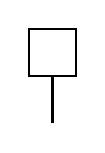
\begin{tikzpicture}[scale=0.3,thick] % , baseline = -3.5pt

\draw (1,1) rectangle (3,3);
\node[anchor=center] (text) at (2,2) {\small $\onehotmapof{\catindex}$};
\draw (2,-1)--(2,1) node[midway,right] {\tiny $\catvariable$};

\end{tikzpicture}
	\end{center}
where $\tilde{\catindex}$ is an indexed represented by an open leg. 
Assigning $\catindex$ to this index will retrieve the $\catindex$th coordinate (with value $1$), whereas all other assignments will retrieve the coordinate values $0$. 


Drawing on the interpretation of tensors by hyeredges we can continue with the definition of tensor networks.

\begin{definition}\label{def:tensorNetwork}
	Let $\graph=(\nodes,\edges)$ be a hypergraph with nodes decorated by categorical variables $\catvariableof{\node}$ with dimensions
		\[ \catdimof{\node} \in \nn \]	
	and hyperedges $\edge\in\edges$ decorated by core tensors
		\[ \hypercoreofat{\edge}{\catvariableof{\edge}} \in \bigotimes_{\node\in\edge}\rr^{\catdimof{\node}} \, , \]
	where we denote by $\catvariableof{\edge}$ the set of categorical variables $\catvariableof{\node}$ with $\node\in\edge$.
	Then we call the set 
		\[ \tnetofat{\graph}{\catvariableof{\nodes}} = \{\hypercoreofat{\edge}{\catvariableof{\edge}}  \, : \, \edge\in\edges\} \]
	the Tensor Network of the decorated hypergraph $\graph$.
\end{definition}


\begin{figure}
	\begin{center}
		\begin{tikzpicture}[scale=0.35,thick] % , baseline = -3.5pt


\node[anchor=center] (text) at (-2,0) {$a)$};

\node [circle, draw, thick, fill=gray!50, minimum size = \nodeminsize] (P1) at (0,-3) {\tiny $\catvariableof{0}$};	
\node [circle, draw, thick, fill=gray!50, minimum size = \nodeminsize] (P2) at (3,-3) {\tiny $\catvariableof{1}$};
\node [circle, draw, thick, fill=gray!50, minimum size = \nodeminsize] (P3) at (6,-3) {\tiny $\catvariableof{2}$};

\node [circle, draw, thick, fill=gray!50, minimum size = \nodeminsize] (P4) at (9,-3) {\tiny $\catvariableof{3}$};;


\draw (P1) to[bend right=-20] (3,0);
\draw (P2) to[bend right=0] (3,0);
\draw (P3) to[bend right=20] (3,0);
\node[anchor=center] (text) at (3,0.5) {$\edge_0$};

\draw (P2) to[bend right=20] (4.5,-6);
\draw (P3) to[bend right=-20] (4.5,-6);

\node[anchor=center] (text) at (4.5,-6.5) {$\edge_1$};

\draw (P3) to[bend right=20] (7.5,-6);
\draw (P4) to[bend right=-20] (7.5,-6);

\node[anchor=center] (text) at (7.5,-6.5) {$\edge_2$};


\begin{scope}[shift={(25,0)}]

\node[anchor=center] (text) at (-2,0) {$b)$};

\draw (-1,-1) rectangle (5,-3);
\node[anchor=center] (text) at (2,-2) {\small $\hypercoreof{\edge_0}$};
\draw (0,-3)--(0,-5) node[midway,left] {\tiny $\catlegof{0}$}; 
\draw (2,-3)--(2,-5) node[midway,left] {\tiny $\catlegof{1}$}; 
%\draw (3,-3)--(3,-5) node[midway,left] {\tiny $\catlegof{1}$}; 
\draw (4,-3)--(4,-5) node[midway,left] {\tiny $\catlegof{2}$}; 


\draw (6,-1) rectangle (10,-3);
\node[anchor=center] (text) at (8,-2) {\small $\hypercoreof{\edge_2}$};
\draw (7,-3)--(7,-5) node[midway,right] {\tiny $\catlegof{2}$}; 
\draw (9,-3)--(9,-5) node[midway,right] {\tiny $\catlegof{3}$}; 


\draw (1,-7) rectangle (5,-9);
\node[anchor=center] (text) at (3,-8) {\small $\hypercoreof{\edge_1}$};
\draw (2,-5)--(2,-7); % node[midway,left] {\tiny $\catlegof{1}$}; 
\draw (4,-5) to[bend right=20]  (7,-6); % node[midway,left] {\tiny $\catlegof{2}$}; 
\draw (4,-7) to[bend right=-20]  (7,-6); 

\draw[fill] (2,-6) circle (0.25cm);
\draw (2,-6) to[bend right=20] (-1,-8); % node[midway, right]{\tiny $\catlegof{1}$};
\node[anchor=center] (text) at (-2,-8) {\tiny $\catlegof{1}$};

\draw[fill] (7,-6) circle (0.25cm);
\draw (7,-5) -- (7,-6);
\draw (7,-6)--(7,-8) node[midway,right] {\tiny $\catlegof{2}$}; 

\end{scope}


\end{tikzpicture}
	\end{center}
	\caption{
	Example of a tensor network.
	a) Hypergraph with edges $\edge_0=\{\catvariableof{0},\catvariableof{1},\catvariableof{2}\}$, $\edge_1=\{\catvariableof{1},\catvariableof{2}\}$ and $\edge_2=\{\catvariableof{2},\catvariableof{3}\}$ decorated by tensor cores.
	b) Dual tensor network, depicting a contraction with leaving all variables open.
	}\label{fig:network}
\end{figure}

%%
%Diagrammatic notation: Best to do version a) as used in the definition, highlighting that tensors have shared categorical variables with fixed dimensions.




\subsubsection{Tensor Product}

% Diagrams -> Contractions
Let us now exploit the developed graphical representations to define contractions of tensor networks.
The simplest contraction is the tensor product, which maps a pair of two tensors with distinct variables onto a third tensor and has an interpretation by coordinatewise products.
Such a contraction corresponds with a tensor network of two tensors with disjoint variables, depicted as:
\begin{center}
	\begin{tikzpicture}[scale=0.35,thick] % , baseline = -3.5pt


\begin{scope}[shift={(-15,0)}]



\draw (-1,1) rectangle (10,-1);
\node[anchor=center] (text) at (4.5,0) {\corelabelsize $\hypercoreof{\edge_0}$};

\draw (0,-1)--(0,-3) node[midway,left] {\colorlabelsize $\catvariableof{0}$};
\draw (3,-1)--(3,-3) node[midway,left] {\colorlabelsize $\catvariableof{1}$};
\node[anchor=center] (text) at (3,-4) {$\cdots$};
\draw (9,-1)--(9,-3) node[midway,right] {\colorlabelsize $\catvariableof{\atomorder\shortminus1}$};

\node [circle, draw, thick, fill=\nodegrayscale, minimum size = \nodeminsize] (P1) at (0,-4) {\colorlabelsize $\catvariableof{0}$};
\node [circle, draw, thick, fill=\nodegrayscale, minimum size = \nodeminsize] (P2) at (3,-4) {\colorlabelsize $\catvariableof{1}$};
\node[anchor=center] (text) at (6,-4) {$\cdots$};

\node [circle, draw, thick, fill=\nodegrayscale, minimum size = \nodeminsize] (P3) at (9,-4) {};

\node[anchor=center] (text) at (9,-4) {\colorlabelsize $\catvariableof{\atomorder-1}$};



\end{scope}




\draw (-1,1) rectangle (10,-1);
\node[anchor=center] (text) at (4.5,0) {\corelabelsize $\hypercoreof{\edge_1}$};

\draw (0,-1)--(0,-3) node[midway,left] {\colorlabelsize $\seccatvariableof{0}$};
\draw (3,-1)--(3,-3) node[midway,left] {\colorlabelsize $\seccatvariableof{1}$};
\node[anchor=center] (text) at (3,-4) {$\cdots$};
\draw (9,-1)--(9,-3) node[midway,right] {\colorlabelsize $\seccatvariableof{\seccatorder\shortminus1}$};

\node [circle, draw, thick, fill=\nodegrayscale, minimum size = \nodeminsize] (P1) at (0,-4) {\colorlabelsize $\seccatvariableof{0}$};
\node [circle, draw, thick, fill=\nodegrayscale, minimum size = \nodeminsize] (P2) at (3,-4) {\colorlabelsize $\seccatvariableof{1}$};
\node[anchor=center] (text) at (6,-4) {$\cdots$};

\node [circle, draw, thick, fill=\nodegrayscale, minimum size = \nodeminsize] (P3) at (9,-4) {};

\node[anchor=center] (text) at (9,-4) {\colorlabelsize $\seccatvariableof{\seccatorder-1}$};




\end{tikzpicture}
\end{center}

\begin{definition}[Tensor Product]\label{def:tensorProduct}
	Let there be two tensor
	\begin{align*}
		\hypercoreofat{\edge_0}{\shortcatvariables} : \facstates \rightarrow \rr \quad \text{and} \quad  \hypercoreofat{\edge_1}{\secshortcatvariables} : \secfacstates \rightarrow \rr \, 
	\end{align*}
	with different categorical variables assigned to its axes.
	Then there tensor product is the map
	\begin{align*}
		\contractionof{\hypercoreofat{\edge_0}{\shortcatvariables},\hypercoreofat{\edge_1}{\secshortcatvariables}}{\shortcatvariables,\secshortcatvariables} :  \left(\facstates\right) \times \left(\secfacstates\right) \rightarrow \rr
	\end{align*}
	defined for $\catindices\in\facstates$ and $\seccatindices\in\secfacstates$ as
	\begin{align*}
		& \contractionof{\hypercore,\sechypercore}{\indexedcatvariables,\indexedseccatvariables} \\
		&\quad\quad :=  \hypercoreofat{\edge_0}{\indexedcatvariables}\cdot \hypercoreofat{\edge_1}{\indexedseccatvariables} \, .
	\end{align*}
\end{definition}

% Other notations
Other popular standard notations of tensor products (see \cite{kolda_tensor_2009,hackbusch_tensor_2012,cichocki_tensor_2015}) 
	\[ \left(\hypercore \otimes \sechypercore\right) = \left(\hypercore \circ \sechypercore\right)  
	= \contractionof{\hypercoreofat{\edge_0}{\shortcatvariables},\hypercoreofat{\edge_1}{\secshortcatvariables}}{\shortcatvariables,\secshortcatvariables}  \, . \]
We will avoid these notations in this work in favor of a consistent notation capable of depicting generic tensor network contractions.

When the tensor $\hypercoreofat{\edge_1}{\secshortcatvariables}$ coincides with the trivial tensor $\onesat{\secshortcatvariables}$ (see Example~\ref{exa:trivialTensor}), we further make a notation convention to omit that tensor, that is
\begin{align*}
	\contractionof{\hypercoreofat{\edge_0}{\shortcatvariables},\onesat{\secshortcatvariables}}{\shortcatvariables,\secshortcatvariables}  
	= \contractionof{\hypercoreofat{\edge_0}{\shortcatvariables}}{\shortcatvariables,\secshortcatvariables} \, .
\end{align*}


\subsubsection{Generic Contractions}


Contractions of Tensor Networks $\extnet$ are operations to retrieve single tensors by summing products of tensors in a network over common indices.
We will define contractions formally by specifying just the indices not to be summed over.

When some of the variables are not appearing as leg variables, we define the contraction as being a tensor product with the trivial tensor $\ones$ carrying the legs of the missing variables.

\begin{definition}\label{def:contraction}
	Let $\tnetof{\graph}$ be a tensor network on a decorated hypergraph $\graph=(\nodes,\edges)$.
	For any subset $\secnodes\subset\nodes$ we define the contraction  to be the tensor 
	\begin{align}
		\contractionof{\tnetof{\graph}}{\catvariableof{\secnodes}} \in \bigotimes_{\node\in\secnodes} \rr^{\catdimof{\node}}
	\end{align}
	defined coordinatewise by the sum	
	\begin{align}
		\contractionof{\tnetof{\graph}}{\indexedcatvariableof{\secnodes}} =
		\sum_{\catindexof{\nodes/\secnodes} \in\,\nodestatesof{\nodes/\secnodes}}
		\left( \prod_{\edge\in\edges}\hypercoreofat{\edge}{\indexedcatvariableof{\edge}} \right) \, .
	\end{align}
	We call $\catvariableof{\secnodes}$ the open variables of the contraction.
\end{definition}


\begin{figure}
	\begin{center}
		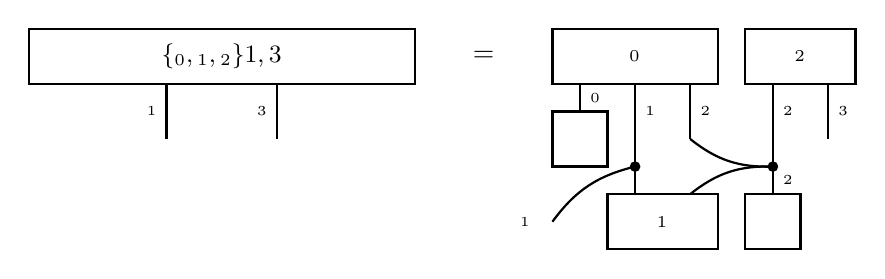
\begin{tikzpicture}[scale=0.35,thick] % , baseline = -3.5pt


%\node[anchor=center] (text) at (-2,0) {$a)$};

\draw (-5,-1) rectangle (9,-3);
\node[anchor=center] (text) at (2,-2) {\small $\contractionof{\{\hypercoreof{\edge_0},\hypercoreof{\edge_1},\hypercoreof{\edge_2}\}}{\catvariableof{1},\catvariableof{3}}$};
\draw (0,-3)--(0,-5) node[midway,left] {\tiny $\catvariableof{1}$}; 
\draw (4,-3)--(4,-5) node[midway,left] {\tiny $\catvariableof{3}$}; 

\node[anchor=center] (text) at (11.5,-2) {${=}$};

\begin{scope}[shift={(15,0)}]

%\node[anchor=center] (text) at (-2,0) {$b)$};

\draw (-1,-1) rectangle (5,-3);
\node[anchor=center] (text) at (2,-2) {\small $\hypercoreof{\edge_0}$};
\draw (0,-3)--(0,-4) node[midway,right] {\tiny $\catvariableof{0}$}; 
\draw (-1,-4) rectangle (1,-6);
\node[anchor=center] (text) at (0,-5) {\small $\ones$};

\draw (2,-3)--(2,-5) node[midway,right] {\tiny $\catvariableof{1}$}; 
\draw (4,-3)--(4,-5) node[midway,right] {\tiny $\catvariableof{2}$}; 


\draw (6,-1) rectangle (10,-3);
\node[anchor=center] (text) at (8,-2) {\small $\hypercoreof{\edge_2}$};
\draw (7,-3)--(7,-5) node[midway,right] {\tiny $\catvariableof{2}$}; 
\draw (9,-3)--(9,-5) node[midway,right] {\tiny $\catvariableof{3}$}; 


\draw (1,-7) rectangle (5,-9);
\node[anchor=center] (text) at (3,-8) {\small $\hypercoreof{\edge_1}$};
\draw (2,-5)--(2,-7); % node[midway,left] {\tiny $\catvariableof{1}$}; 
\draw (4,-5) to[bend right=20]  (7,-6); % node[midway,left] {\tiny $\catvariableof{2}$}; 
\draw (4,-7) to[bend right=-20]  (7,-6); 

\draw[fill] (2,-6) circle (0.15cm);
\draw (2,-6) to[bend right=20] (-1,-8); % node[midway, right]{\tiny $\catvariableof{1}$};
\node[anchor=center] (text) at (-2,-8) {\tiny $\catvariableof{1}$};

\draw[fill] (7,-6) circle (0.15cm);
\draw (7,-5) -- (7,-6);
\draw (7,-6)--(7,-7) node[midway,right] {\tiny $\catvariableof{2}$}; 

\draw (6,-7) rectangle (8,-9);
\node[anchor=center] (text) at (7,-8) {\small $\ones$};

\end{scope}


\end{tikzpicture}
	\end{center}
	\caption{
		Example of a tensor network contraction of all but the variables $\catvariableof{1},\catvariableof{3}$.
		Contraction of variables can always be depicted by closing the open legs with trivial tensors $\ones$ performing index sums.
	}\label{fig:contraction}
\end{figure}

%%
%Diagrammatic notation: Best to do version b), since this is easiest to see how tensors combine to new tensors by contractions.

\begin{remark}[Alternative Notations]
	% Einstein summations
	Contractions can also denoted by the Einstein summations of the indices along connected edges, understood as scalar product in each subspace.
	This is as in \defref{def:contraction}, just omitting the sums.
	We found it useful in this work to do the diagrammatic representation instead, since it offers a better possibility to depict hierarchical arrangements of shared variables.
\end{remark}


% Mode products
Further notations without usage of axis variables are mode products (see \cite{kolda_tensor_2009,hackbusch_tensor_2012,cichocki_tensor_2015}), often denoted by the operation $\times_n$.
With our more generic variable-based notations, we can capture these more specific contractions by coloring the tensor axes, that is assignment of axis variables.

% Examples
To further gain familiarity with the generic contractions, we show the connection to two more popular examples.

%% Diagrammatic representation of Matrix Vector
\begin{example}{Matrix Vector Products}
	The matrix vector product is a special case of tensor contractions, where a matrix $\matrixat{\exrandom,\secexrandom}$ shares a categorical variable with a vector $\vectorat{\secexrandom}$.
	When leaving the variable unique to the matrix open we get the matrix vector product as
		\[ \contractionof{\matrixat{\exrandom,\secexrandom},\vectorat{\secexrandom}}{\exrandom=\exrandind} = \sum_{\secexrandind\in[\secexranddim]} \matrixat{\exrandom=\exrandind,\secexrandom=\secexrandind} \cdot \vectorat{\secexrandom=\secexrandind} \, .  \]

	Exploiting the diagramatic tensor network visualization we depict matrix vector products by:
	\begin{center}
		\begin{tikzpicture}[scale=0.3,thick,xscale=-1] % , baseline = -3.5pt

\draw (-9,2)--(-7,2) node[midway,above] {\colorlabelsize $\exrandom$};
\draw (-21,1) rectangle (-9,3);
\node[anchor=center] (text) at (-15,2) {\corelabelsize $\contractionof{\matrixat{\exrandom,\secexrandom},\vectorat{\secexrandom}}{\exrandom}$};

\node[anchor=center] (text) at (-5,2) {\corelabelsize ${=}$};

\draw (3,2)--(5,2) node[midway,above] {\colorlabelsize $\exrandom$};
\draw (1,1) rectangle (3,3);
\node[anchor=center] (text) at (2,2) {\corelabelsize $\exmatrix$};
\draw (1,2)--(-1,2) node[midway,above] {\colorlabelsize $\secexrandom$};
\draw (-1,1) rectangle (-3,3);
\node[anchor=center] (text) at (-2,2) {\corelabelsize $\exvector$};

%\node[anchor=center] (text) at (7,1) {$\cdot$};


\end{tikzpicture}
	\end{center}
%	Here the index $j$ is represented by a closed edge, which means that it is eliminated by a sum.
\end{example}


%% Hadamard Product 
\begin{example}{Hadamard Products of Vectors}
	A node appearing in arbitrary many hyperedges denotes a Hadamard product of the axis of the respective decorating tensors.
	To give an example, let $\vectorofat{\catenumerator}{\catvariable}\in\rr^\catdim$ be vectors for $\catenumeratorin$. Their hadamard product is the vector
		\[ \contractionof{\{\vectorofat{\catenumerator}{\catvariable} \, : \, \catenumeratorin\}}{\catvariable}  \in \rr^\catdim \]
	defined by
		\[ \contractionof{\{\vectorofat{\catenumerator}{\catvariable} \, : \, \catenumeratorin\}}{\indexedcatvariable}   
		= \prod_{\atomenumeratorin} \vectorofat{\atomenumerator}{\indexedcatvariable}\, . \]
	In a contraction diagram the Hadamard product is depicted by 
	\begin{center}
		\begin{tikzpicture}[scale=0.3,thick] % , baseline = -3.5pt


\begin{scope}[shift={(-10,0)}]

\draw (-5,1) rectangle (7,3);
\node[anchor=center] (text) at (1,2) {\small $\contractionof{V^{0}[\catvariable],\ldots,V^{\catorder-1}[\catvariable]}{\catvariable}$}; % {\small $\contractionof{\{\vectorofat{\catenumerator}{\catvariable} \, : \, \catenumeratorin\}}{\catvariable}$};
\draw (1,-1)--(1,1) node[midway,right] {\tiny $\catvariable$};

\node[anchor=center] (text) at (9,2) {${=}$};

\end{scope}



\draw (1,1) rectangle (3,3);
\node[anchor=center] (text) at (2,2) {\small $\vectorof{0}$};
\draw (2,-1)--(2,1) node[midway,right] {\tiny $\catvariable$};


\begin{scope}[shift={(5,0)}]

\draw (1,1) rectangle (3,3);
\node[anchor=center] (text) at (2,2) {\small $\vectorof{1}$};
\draw (2,-1)--(2,1) node[midway,right] {\tiny $\catvariable$};

\end{scope}

\node[anchor=center] (text) at (11.5,2) {\small $\cdots$};


\begin{scope}[shift={(15,0)}]

\draw (0.75,1) rectangle (3.25,3);
\node[anchor=center] (text) at (2,2) {\small $\vectorof{\atomorder\shortminus1}$};
\draw (2,-1)--(2,1) node[midway,right] {\tiny $\catvariable$};

\end{scope}


\draw[fill] (9.125,-4.5) circle (0.15cm);

\draw (9.125,-4.5) to[bend right=-20] (2,-1); 
\draw (9.125,-4.5) to[bend right=-20] (7,-1); 
\draw (9.125,-4.5) to[bend right=20] (17,-1); 

\draw (9.125,-4.5) -- (9.125,-6.5) node[midway,right] {\tiny $\catvariable$};; 

\end{tikzpicture}
	\end{center}
\end{example}



\subsubsection{Decompositions}

Tensors can be represented by tensor network decompositions, when the contraction of the network retrieves the tensor.

\begin{definition}\label{def:tnDecomposition}
	%Let $\hypercoreat{\nodevaraibles}$ be a tensor in $\extensorspace$.
	A Tensor Network Decomposition of a tensor $\hypercoreat{\nodevariables}$ is a Tensor Network $\tnetof{\graph}$ such that
		\[ \hypercoreat{\nodevariables}= \contractionof{\tnetof{\graph}}{\nodevariables} \, . \]
	We call the hypergraph $\graph$ the format of the decomposition.
\end{definition}



\subsection{Properties of Tensors}

%% Boolean
We will often encounter situations, where the coordinates of tensors are in $\{0,1\}=[2]$.

\begin{definition}\label{def:booleanTensor} % CALL BOOLEAN INSTEAD?
	We call a tensor $\hypercoreat{\shortcatvariables}$ boolean, when $\imageof{\hypercore}\subset[2]$, i.e. all coordinates are either $0$ or $1$.
\end{definition}

%% Directionality
Directionality represents constraints on the structure of tensors:
Summing over outgoing trivializes the tensor.

\begin{definition}\label{def:directedTensor}
	A Tensor 
		\[ \hypercoreat{\nodevariables} \in \bigotimes_{\nodein}\rr^{\catdimof{\node}} \]
	is said to be directed with incoming variables $\innodes$ and outgoing variables $\outnodes$, where $\nodes=\innodes\dot{\cup}\outnodes$, when
		\[ \sbcontractionof{\hypercore}{\catvariablesinset{\outnodes}} =  \onesat{\catvariablesinset{\innodes}} \]
	where $\onesat{\catvariablesinset{\innodes}}$ denoted the trivial tensor in  $\bigotimes_{\node\in\innodes}\rr^{\catdimof{\node}}$ which coordinates are all $1$.
\end{definition}

While by default all legs are outgoing, we can change the direction by normation.

\begin{definition}\label{def:normation}
	A tensor $\hypercoreat{\nodevariables}$ is said to be normable on $\innodes\subset\nodes$, if for any $\catindexof{\innodes}\in\nodestatesof{\innodes}$ we have
		\[ \sbcontraction{\hypercoreat{\nodevariables},\onehotmapofat{\atomlegindexof{\innodes}}{\catvariableof{\innodes}}} > 0 \, . \]
	The normation of a on $\innodes\subset\nodes$ normable tensor is the tensor
	\begin{align*}
		\sbnormationofwrt{\hypercoreat{\nodevariables}}{\catvariableof{\outnodes}}{\catvariableof{\innodes}} = 
		\sum_{\catindexof{\innodes}\in\nodestatesof{\innodes}} 
		\onehotmapofat{\atomlegindexof{\innodes}}{\catvariableof{\innodes}} \otimes \frac{
		\sbcontractionof{\hypercoreat{\nodevariables},\onehotmapofat{\catindexof{\innodes}}{\catvariableof{\innodes}}}{\catvariableof{\outnodes}}
		}{
		\sbcontraction{\hypercoreat{\nodevariables},\onehotmapofat{\catindexof{\innodes}}{\catvariableof{\innodes}}}
		} 
	\end{align*}
	where $\outnodes = \nodes/\innodes$.
\end{definition}

We will investigate the contractions of directed tensors in \parref{par:three}, where we show in Theorem~\ref{the:normationDirected} that normations are directed tensors.


%% Diagrammatic notation
In our graphical tensor notation, we depict directed tensors by directed hyperedges (a), which are decorated by directed tensors (b), for example:
%\red{Draw incoming and outgoing example.}
	\begin{center}
		


\begin{tikzpicture}[scale=0.35,thick] % , baseline = -3.5pt

\node[anchor=center] (text) at (-2,0) {$a)$};

\node [circle, draw, thick, fill=\nodegrayscale, minimum size = \nodeminsize] (P1) at (0,-3) {\colorlabelsize $\catvariableof{0}$};
\node [circle, draw, thick, fill=\nodegrayscale, minimum size = \nodeminsize] (P2) at (3,-3) {\colorlabelsize $\catvariableof{1}$};

%\node[anchor=center] (text) at (6,-3) {$\cdots$};
\node [circle, draw, thick, fill=\nodegrayscale, minimum size = \nodeminsize] (P3) at (6,-3)  {\colorlabelsize $\catvariableof{2}$};

\node [circle, draw, thick, fill=\nodegrayscale, minimum size = \nodeminsize] (P4) at (9,-3)  {\colorlabelsize $\catvariableof{3}$};

\node[anchor=center] (text) at (9,-3) {\colorlabelsize $\catvariableof{3}$};


\draw[midarrow] 
    	(4.5,0) to[bend right=25] (P1);
\draw[midarrow] 
    	(4.5,0) to[bend right=10] (P2);
\draw[midarrow] 
    	(P3) to[bend right=10] (4.5,0);
\draw[midarrow] 
	(P4) to[bend right=25] (4.5,0);
	
\node[anchor=center] (text) at (4.5,0.5) {$\edge$};


\begin{scope}[shift={(20,0)}]

\node[anchor=center] (text) at (-2,0) {$b)$};

\draw (-1,-1) rectangle (7,-3);
\node[anchor=center] (text) at (3,-2) {\corelabelsize $\hypercoreofat{\edge}{\catvariableof{0},\catvariableof{1},\catvariableof{2},\catvariableof{3}}$};
%\draw[->-] (0,-3)--(0,-5) node[midway,left] {\colorlabelsize $\catvariableof{0}$};
%\draw[->-] (1.5,-3)--(1.5,-5) node[midway,left] {\colorlabelsize $\catvariableof{1}$};
%\node[anchor=center] (text) at (3,-4) {$\cdots$};
%\draw[->-] (4,-3)--(4,-5) node[midway,right] {\colorlabelsize $\catvariableof{\atomorder-1}$};


\draw[midarrow]  (0,-3) -- (0,-5) node[midway,left] {\colorlabelsize $\catvariableof{0}$};
\draw[midarrow] 
    (2,-3)--(2,-5) node[midway,left] {\colorlabelsize $\catvariableof{1}$};
\draw[midarrow] 
    (4,-5)--(4,-3) node[midway,left] {\colorlabelsize $\catvariableof{2}$};
\draw[midarrow] 
   (6,-5)--(6,-3) node[midway,right] {\colorlabelsize $\catvariableof{3}$};
\end{scope}



\end{tikzpicture}
	\end{center}



\subsection{Encoding schemes for functions}

Tensors are defined here as real-valued functions on the state set of a system described by categorical variables.
We provide further schemes to represent functions in order to perform sparse calculus and to handle more generic functions.



%
%\subsubsection{Real-valued functions}
%\begin{example}[Uncertainty about States]\label{exa:onehotUncertainty}
%	The uncertainty about the state of a categorical variable $\catvariable$ can be expressed in vectors.
%	For example let there be real numbers $\probof{\catvariable=\catindex} \in [0,1]$ for $\catindex\in[\catdim]$ with $\sum_{\catindex\in[\catdim]}\probof{\catvariable=\catindex}=1$ with the interpretation that $\probof{\catvariable=\catindex}$ is the probability of a system being in state $\catindex$. 
%	We can represent this uncertain state simply by a vector 
%		\[ \probof{\catvariable}\in\rr^{\catdim} \]
%	defined as the sum of one-hot representations weighted by $\probof{\catvariable=\catindex}$
%	\[ \sum_{\catindex\in[\catdim]} \probof{\catvariable=\catindex} \cdot \onehotmapofat{\catindex}{\catvariable} =
%		\begin{bmatrix}
%		\probof{\catvariable=0} & \probof{\catvariable=1} & \cdots & \probof{\catvariable=\catdim-1}
%		\end{bmatrix} \, . 
%	\]
%\end{example}



\subsubsection{Relational encodings}

%We have already observed in Example~\ref{exa:atomicFunction}, that any function of a categorical variable has a representation as a linear function acting on the one-hot encoding of the variable.
Let us now show how we can encode maps between factored systems.
The scheme is described in more generality and detail (encoding of subsets and relations) in \charef{cha:basisCalculus}, see \defref{def:functionRelationEncoding}.

\begin{definition}[Relation encoding of maps between Factored Systems]\label{def:functionRepresentation}
	Let $\exfunction$ be a function
		\[ \exfunction : \facstates \rightarrow  \secfacstates \]
	which maps the states of a factored system to variables $\catvariables$ to the states of another factored system with variables $\seccatvariables$.
	Then the tensor representation of $\exfunction$ is a tensor
		\[ \rencodingofat{\exformula}{\catvariables,\seccatvariables} \in  \left(\secfacspace\right) \otimes \left(\facspace\right)  \]
	defined by
		\[ \rencodingofat{\exformula}{\seccatvariables,\catvariables}= \sum_{\catindices\in\facstates}  
		\onehotmapofat{\exfunction(\catindices)}{\seccatvariables} \otimes  \onehotmapofat{\catindices}{\catvariables} \, . \]
\end{definition}

We depict relational encodings by directed tensors:
\begin{center}
	\begin{tikzpicture}[scale=0.35,thick] % , baseline = -3.5pt


\draw[->] (0,-1)--(0,1) node[midway,left] {\tiny $\headvariableof{0}$}; 
\draw[->] (1.5,-1)--(1.5,1) node[midway,left] {\tiny $\headvariableof{1}$}; 
\node[anchor=center] (text) at (3,-4) {$\cdots$};
\draw[->] (4,-1)--(4,1) node[midway,right] {\tiny $\headvariableof{\seccatorder\shortminus1}$}; 

\draw (-1,-1) rectangle (5,-3);
\node[anchor=center] (text) at (2,-2) {\small $\rencodingof{\exfunction}$};
\draw[<-] (0,-3)--(0,-5) node[midway,left] {\tiny $\catvariableof{0}$}; 
\draw[<-] (1.5,-3)--(1.5,-5) node[midway,left] {\tiny $\catvariableof{1}$}; 
\node[anchor=center] (text) at (3,-4) {$\cdots$};
\draw[<-] (4,-3)--(4,-5) node[midway,right] {\tiny $\catvariableof{\atomorder\shortminus1}$}; 


%\drawatomcore{3.5}{-8}{$\probtensor$}
%\drawatomindices{3.5}{-12}	
%\draw (5.5,-9)--(5.5,-7) node[midway,right] {\tiny $\catvariableof{\exformula}$};

\end{tikzpicture}
\end{center}


% Notation with image categorical variable
%When the categorical variables of the image factored system to a map $\exfunction$ are not specified otherwise, we will denote them by $\catvariableof{\exfunction}$.




\subsubsection{Tensor-valued functions}


%% TO DETAILLED HERE -> Part III?
\begin{definition}[Selection encoding of Maps between Factored Systems]\label{def:selectionEncoding}
	Given a tensor space $\parspace$ described by categorical variables $\selvariables$ and a tensor-valued function
		\[ \exfunction : \facstates \rightarrow \parspace \]
	the selection encoding of $\exfunction$ is a tensor
		\[ \sencodingofat{\exfunction}{\shortcatvariables,\shortselvariables} \in \left(\facspace\right) \otimes \left(\parspace\right) \]
	defined by the basis decomposition
		\[ \sencodingofat{\exfunction}{\shortcatvariables,\shortselvariables} = \sum_{\catindices\in\facstates} \onehotmapofat{\catindices}{\shortcatvariables} \otimes \exfunction(\catindices)[\shortselvariables] \, .  \]
\end{definition}

%%
We call these tensor representation of maps selection encodings, since the coordinate of a function $\exfunction$ to be processed is selected by another argument to $\sencodingof{\exfunction}$.

%\begin{example}[Vector valued functions]\label{exa:atomicFunction} %% CONFUSIN, since already needs selection variables?
%	When using a one-hot representation of the state of a categorical variable, any real valued function has a representation by a real valued matrix acting on the one-hot encoding. 
%	Let there be a vector valued function
%		\[ \exformula : [\catdim] \rightarrow \rr^p \]
%	which maps $\catindex\in[\catdim]$ to the vector
%		\[ \exformula(\catindex)[\selvariable] \in \rr^p \, , \]
%	where we introduced the variable $\selvariable\in[p]$ selecting a coordinate of the image vector.
%	The 
%		\[ \exformula(\catindex)[\selvariable] = 
%		\contractionof{\{\onehotmapof{\catindex}[\catvariable] , \,\concore_{\exformula}[\catvariable,\selvariable]\}}{\selvariable}  \]
%	where $\concore_{\exformula} \in \rr^{\catdim \times p} $ is the matrix defined by the function evaluation vectors of $\exformula$ as
%		\[ \concore_{\exformula}[\catvariable,\selvariable] = \begin{bmatrix}
%			-- & \exformula(0) & -- \\
%			-- & \exformula(1) & -- \\
%			& \vdots &  \\
%			-- & \exformula(\catdim-1) & -- 
%		\end{bmatrix} \, . 
%		\]
%	This can easily be verified, since matrix multiplication with basis vectors amounts to selection of rows (when the basis vector is acting from the left) or columns (when the basis vector is acting from the right).
%	Thus, linear transforms (matrices) acting on the one-hot representation are sufficient to represent any vector valued function of the states of a categorical variable.
%\end{example} 


%% 
We will provide more detail to the tensor representation of functions in \parref{par:three}, where we distinguish between embeddings for basis and coordinate calculus. %where we show that domain encodings coincide with selection encodings.





